\documentclass[xcolor={dvipsnames}]{beamer}
\mode<presentation>{\usetheme{boxes}}
\usecolortheme{default}
\setbeamertemplate{navigation symbols}{}%remove navigation symbols

\setbeamerfont{frametitle}{size=\Large}

%\setbeamercolor{structure}{fg=beamer@blendedblue}



\setbeamertemplate{bibliography item}{\insertbiblabel}

\setbeamercolor{bibliography entry author}{fg=black}
\setbeamercolor{bibliography entry title}{fg=black} 
\setbeamercolor{bibliography entry location}{fg=black} 
\setbeamercolor{bibliography entry note}{fg=black}  

\usepackage[style=numeric,sorting=ydnt,maxnames=1,defernumbers=true, firstinits=true]{biblatex}
\renewbibmacro{in:}{}
\ExecuteBibliographyOptions{sorting=ydnt}

%\addbibresource{./jlescSummerSchool_checkpointing.bib}

\makeatother
\setbeamertemplate{footline}
{
  \leavevmode%
  \hbox{%
    %% \begin{beamercolorbox}[wd=.2\paperwidth,ht=2.25ex,dp=1ex]{date in head/foot}%
    %%   \usebeamerfont{date in foot}
    %% \end{beamercolorbox}%
  %%   \begin{beamercolorbox}[wd=.6\paperwidth,ht=2.25ex,dp=1ex, center]{date in head/foot}%
  %%     \usebeamerfont{date in foot}\insertshortdate
  %% \end{beamercolorbox}%
  \begin{beamercolorbox}[wd=\paperwidth,ht=2.25ex,dp=1ex]{date in head/foot}%
    \usebeamerfont{date in foot}\hfill
    {\scriptsize\insertframenumber{}}\hspace*{2ex}
  \end{beamercolorbox}}%
  \vskip0pt%
}
\makeatletter



\usepackage[utf8]{inputenc}
%\usepackage[T1]{fontenc}
%\usepackage[francais]{babel}
\usepackage{hyperref}
\usepackage{url}
\usepackage{pifont}
\usepackage{changepage}
\usepackage{listings}
\lstset{basicstyle=\ttfamily,
  showstringspaces=false,
  commentstyle=\color{black},
  keywordstyle=\color{black}
}

\usepackage{fancyvrb}
\usepackage{multirow}
\usepackage{tabu} 
\usepackage{colortbl}

\usepackage{marvosym}

\usepackage{eurosym}

%\usepackage{gitdags}
\usepackage{comment}

\usepackage{pdfpages}
\setbeamercolor{background canvas}{bg=}


\usepackage{perpage} %the perpage package
\MakePerPage{footnote}



\definecolor{beamer@blendedblue}{RGB}{0,102,204}

\definecolor{beamer@lightgray}{RGB}{238,238,224}


\definecolor{itemorange}{RGB}{255,114,0}


\definecolor{myorange}{RGB}{255,103,0}


\setbeamertemplate{itemize items}[circle]
\setbeamertemplate{itemize subitem}[triangle]


\setbeamercolor{itemize item}{fg=beamer@blendedblue}
\setbeamercolor{itemize subitem}{fg=gray}


\newcommand<>{\Blue}[1]{{\color#2{beamer@blendedblue}#1}}
%\newcommand<>{\Orange}[1]{{\color#2{BurntOrange}#1}}
\newcommand<>{\Orange}[1]{{\color#2{myorange}#1}}
\newcommand<>{\Alert}[1]{{\Orange{\textbf{#1}}}}


\newcommand{\largeskip}{\vspace{0.6cm}}
\newcommand{\hugeskip}{\vspace{1cm}}



\usepackage{tikz}
\usetikzlibrary{%
decorations.pathreplacing,%
decorations.pathmorphing,%
decorations.shapes,%
decorations.text,%
decorations.markings,%
shapes,%
shapes.callouts,%
shadows,%
arrows,
calc,%
positioning,%
chains,%
backgrounds,%
fit, %
fadings}

\tikzset{
    invisible/.style={opacity=0},
    visible on/.style={alt={#1{}{invisible}}},
    alt/.code args={<#1>#2#3}{%
      \alt<#1>{\pgfkeysalso{#2}}{\pgfkeysalso{#3}} % \pgfkeysalso doesn't change the path
    },
}


\tikzset{
    colornode/.style={
        outer sep=0pt, fill=#1!67, %text height=2ex, text depth=.5ex
    },
    cpu/.style={
        diamond, fill=gray!30, aspect=3, name=CPU#1,
        node contents={$\text{CPU}_{#1}$},
    },
    thread/.style={fill=#1!67,
        minimum width=5ex, minimum height=1.25em},
    tick/.style={very thin},
}



\newcommand{\email}[1]{\href{mailto:#1}{\nolinkurl{#1}}}

\newcommand{\xmark}{\ding{55}}


\AtBeginPart{
  %\frame{\partpage}
  \frame{
    \frametitle{Agenda}
    \small
    \tableofcontents[part=\insertpartnumber,
    sectionstyle=show,
    subsectionstyle=hide,
    subsubsectionstyle=hide]
  }
}

\AtBeginSection[]
{
  \begin{frame}
    \frametitle{Agenda}
    \small
    \tableofcontents[
    sectionstyle=show/shaded,
    subsectionstyle=show/show/hide,
    subsubsectionstyle=hide]
  \end{frame}
}

\AtBeginSubsection[]{
  \mode<presentation>{
    \frame{\tableofcontents[
      sectionstyle=show/hide,
      subsectionstyle=show/shaded/hide,
      subsubsectionstyle=show/show/hide]
    }
  }
}


\date[\the\year]{\the\year}

\newcommand{\shellcmd}[1]{\indent\indent\texttt{\footnotesize\$ #1}}


\title[]{Cloud Computing}
\subtitle{Concepts de virtualisation\footnote{Adapté du support développé par Thomas ROPARS et Renaud LACHAIZE}}

%Thomas ROPARS : \url{https://tropars.github.io/teaching/},
%\url{https://roparst.gricad-pages.univ-grenoble-alpes.fr/cloud-tutorials/m2gi-devops/}}}


\author[]{\\Danilo Carastan dos Santos
  \\ \vspace{0.5cm} \email{danilo.carastan-dos-santos@univ-grenoble-alpes.fr}}

\definecolor{mybrown}{RGB}{205,133,63}
\definecolor{myblue}{RGB}{28,134,238}

\let\Red=\alert
\newcommand<>{\green}[1]{{\color#2{green!70!black}#1}}
\newcommand<>{\blue}[1]{{\color#2{blue!100!black!100}#1}}
\definecolor{darkgreen}{rgb}{0,0.5,0}

\newcommand\myvdots{{\smash[b]\strut\smash[t]\vdots}}


\usepackage{boxedminipage}
\newenvironment{boitecode}[1]{
    \begin{boxedminipage}{\linewidth}      
%\begin{beamerboxesrounded}[shadow=true,lower=lightex,upper=medex]{#1}
    #1
    \begin{semiverbatim}
}{   \end{semiverbatim}\vspace{-1.5\baselineskip}
    \end{boxedminipage}
%  \end{beamerboxesrounded}
}


\begin{document}


\begingroup
\setbeamercolor{titlelike}{bg=beamer@lightgray, fg=black}
\begin{frame}
\titlepage
\end{frame}
\endgroup

\begin{frame}{Problematique}
    \begin{columns}
        \begin{column}{.4\linewidth}
            
                Applications : 
                \begin{itemize}
                    \item Email
                    \item Partage de données
                \end{itemize}
                Chaque application a de prérequis spécifiques de ressources physiques/logiciels
                \begin{itemize}
                    \item Utilisation de CPU
                    \item Mémoire
                    \item Stockage
                    \item Système d'exploitation
                    \item Librairies/Intergiciels spécifiques
                \end{itemize}            
        \end{column}
        \begin{column}{.6\linewidth}            
            \centering \includegraphics[width=\linewidth]{Figures/data-center-virt-1.pdf}
        \end{column}
    \end{columns}    
\end{frame}

\begin{frame}{Une première solution naïve}
    \begin{columns}
        \begin{column}{.4\linewidth}
            \begin{itemize}
                \item Une application par serveur
                \item Inconvénient : sous-utilisation des serveurs
            \end{itemize}
        \end{column}
        \begin{column}{.6\linewidth}            
            \centering \includegraphics[width=\linewidth]{Figures/data-center-virt-2.pdf}
        \end{column}
    \end{columns}    
\end{frame}

\begin{frame}{Une deuxième solution}
    \begin{columns}
        \begin{column}{.4\linewidth}
            \begin{itemize}
                \item Plusieurs applications par serveur
                \item Problèmes : 
                \begin{itemize}
                    \item Contrôle de ressources
                    \item Isolation d'applications                     
                \end{itemize}
            \end{itemize}
        \end{column}
        \begin{column}{.6\linewidth}            
            \centering \includegraphics[width=\linewidth]{Figures/data-center-virt-3.pdf}
        \end{column}
    \end{columns}   
    Exemple : 
    \begin{itemize}
        \item  Apps A et B tournent dans un même serveur. App A a besoin une
        mise à jour du système d'exploitation. Cette MàJ peut affecter B. 
    \end{itemize} 
\end{frame}

\begin{frame}{Une meilleure solution : virtualisation}

    \begin{itemize}
        \item \textbf{Idée :} Créer plusieurs ressources virtuelles (Machine Virtuelle - VM) à partir
        d'une ou plusieurs ressources physiques        
        \item Dans une VM nous ne pouvons pas distinguer entre ressources
        physiques ou virtuelles
        \item \textbf{Concept clé :} Hyperviseur
        \begin{itemize}
            \item Est une couche logicielle
            \item Fournit l’abstraction d’une ou plusieurs machines ``nues''
            (processeurs, mémoire et périphériques) au-dessus d’une véritable
            machine physique
        \end{itemize}
        \item Intérêt : 
        \begin{itemize}
            \item Faire tourner plusieurs systèmes d’exploitation simultanément
            sur la même plateforme matérielle
            \item Sauvegarder/rembobiner l’état d’un système
            \item Sécurité (renforcement de l’isolation de certaines
            applications)
        \end{itemize}
    \end{itemize} 
\end{frame}

\begin{frame}{Virtualisation}
\begin{itemize}
    \item Hyperviseur de type I (natif) : Couche logicielle de plus bas
    niveau. Système d’exploitation spécialisé. Plus efficace    
    \item Exemples : VMware ESX, Xen
    \item Hyperviseur de type II (hébergé) : Application intermédiaire (intergiciel) qui s’appuie sur un système hôte sous-jacent
    \item Moins efficace (plus de couches) mais plus simple à installer/utiliser
    \item Exemples : VMware workstation/fusion/player, VirtualBox
\end{itemize}

    \centering \includegraphics[width=.7\linewidth]{Figures/virtualisation.pdf}
\end{frame}

\begin{comment}   

\begin{frame}{Image d'une machine virtuelle}
    \begin{itemize}
        \item Snapshot of a virtual machine
        \item Allows for a faster deployment of VMs. No need to install OS +
        additional software every time a vm is launched
    \end{itemize}
    
\end{frame}
\end{comment}

\begin{frame}{Scalabilité}{\textit{Scaling}}
    \begin{itemize}
        \item Terme générique lié au comportement d'une application si la charge
        de travail et/ou les ressources changent
        \item Deux types : 
        \begin{itemize}
            \item \textbf{Scalabilité faible (Weak scaling) :} ``Puis-je faire plus de travail (traiter
            plus de requêtes, traiter plus de données) si j'ai plus de
            ressources ?''  
            \item \textbf{Scalabilité forte (Strong scaling) : } ``Puis-je faire la même charge
            de travail dans moins de temps si j'ai plus de ressources ?''
        \end{itemize}
    \end{itemize}
\end{frame}

\begin{frame}{Elasticité}{\textit{Autoscaling}}
    \begin{itemize}
        \item \textbf{Idée générale : } Adapter les ressources en fonction de la charge de travail courante
        \item Exemple : ``Mon application de commerce électronique basée sur le
        Web devrait traiter n'importe quelle requête en moins de 500 ms, quel
        que soit le nombre total de requêtes qu'elle traite actuellement.''
        \item ``Juste ce qu'il faut'' :
        \begin{itemize}
            \item Pas assez de ressources $\rightarrow$ traitement plus long
            (perte de qualité de service)
            \item Trop de ressources $\rightarrow$ ressources non utilisées (et
            on les paye quand même)
        \end{itemize}
        %\item Pour certains services Cloud, l'Élasticité est transparente pour les utilisateurs
    \end{itemize}
\end{frame}

\begin{frame}{Scalabilité Verticale}{\textit{Vertical Scaling}}

    \begin{columns}
        \begin{column}{.4\linewidth}
            \begin{itemize}
                \item \textbf{Idée : } remplacer les machines (virtuelles) avec des
                machines (virtuelles) plus puissantes
                \item \textbf{Avantages : }
                \begin{itemize}
                    \item Plus simple                    
                \end{itemize}
                \item \textbf{Inconvénients : }
                \begin{itemize}
                    \item Scalabilité limitée 
                    \item Coût non linéaire de ressources                    
                \end{itemize}
            \end{itemize}        
        \end{column}
        \begin{column}{.6\linewidth}            
            \centering 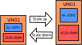
\includegraphics[width=.9\linewidth]{Figures/virtual-scaling.pdf}
        \end{column}
    \end{columns} 
\end{frame}

\begin{frame}{Scalabilité Horizontale}{\textit{Horizontal Scaling}}

    \begin{columns}
        \begin{column}{.4\linewidth}
            \begin{itemize}
                \item \textbf{Idée : } Ajouter plus d'instances de
                l'application. Plusieurs machines virtuelles en parallèle
                \item \textbf{Avantages : }
                \begin{itemize}
                    \item  Système distribué                   
                \end{itemize}
                \item \textbf{Inconvénients : }
                \begin{itemize}
                    \item Plus compliqué à développer : Synchronisation, débogage, etc. 
                                       
                \end{itemize}
            \end{itemize}        
        \end{column}
        \begin{column}{.6\linewidth}            
            \centering \includegraphics[width=.9\linewidth]{Figures/horizontal_scaling.pdf}
        \end{column}
    \end{columns} 
\end{frame}


\begin{frame}{Conteneurs}{\textit{Containers}}
    
    \begin{itemize}
        \item Motivation : Un microservice par VM consomme trop de ressources.
        \begin{itemize}
            \item Par exemple : chaque VM a un OS invité (\textit{guest OS}), ce
            qui est trop pour juste un microservice
        \end{itemize}
        
        \item Démarrage de VM est trop long (plusieurs minutes)
        \begin{itemize}
            \item Il faut démarrer un système complet
        \end{itemize}
        \item Nous souhaitons partager l'OS hôte (\textit{host OS}) entre les
        applications, tout en étant le plus isolé possible.
    \end{itemize}
\end{frame}

\begin{frame}{Conteneurs}{\textit{OS-level virtualization} : comparaison avec Machines Virtuelles}
    \centering 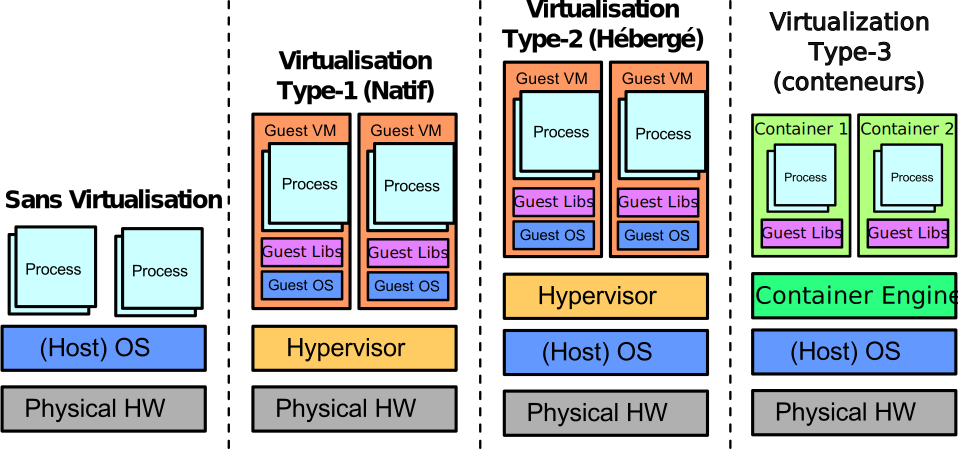
\includegraphics[width=\linewidth]{Figures/virtualisation_full.pdf}
\end{frame}

\begin{frame}{Conteneurs}{\textit{Container Engine} et \textit{Container Runtime}}
    \begin{itemize}
        \item Un environnement d'exécution et un ensemble de services pour
        manipuler des conteneurs docker sur une machine
        \item Exemple : Docker engine
        \item Logiciel client-serveur
        \begin{itemize}
            \item Le serveur -- Un daemon (processus persistant) qui gère les
            conteneurs sur une machine
            \item Le client -- Une interface en ligne de commande
        \end{itemize} 
    \end{itemize}
\end{frame}

\begin{frame}{Conteneurs}{Support du système d'exploitation. Focus sur Linux}
    Plusieurs fonctionnalités fournies par des sous-systèmes et outils du noyau
    Linux pour gérer les conteneurs. Par exemple
        \begin{itemize}
            \item Namespaces\footnote{\url{https://www.man7.org/linux/man-pages/man7/namespaces.7.html}} :
            pour configurer les ressources système visibles par un processus donné
            (interfaces/ports réseau, utilisateurs, PID, etc)
            \item Groupes de contrôle
            (cgroups\footnote{\url{https://www.man7.org/linux/man-pages/man7/cgroups.7.html}}) :
            pour appliquer les limites d'allocation des ressources
            \item Capacités : pour contrôler les opérations qu'un
            processus/utilisateur donné est autorisé à effectuer sur différents
            types de ressources
            \item Seccomp\footnote{\url{https://www.man7.org/linux/man-pages/man2/seccomp.2.html}} :
            pour filtrer les appels système légitimes qu'un processus peut effectuer
        \end{itemize}
        
    \end{frame}

\begin{frame}{Conteneurs}{Concept d'Image}

    Les technologies de conteneurs offrent une solution de \textit{packaging}
pour une application et ses dépendances. 

\textbf{Les images de conteneurs : } Package de l'application et de ces
dépendances

\begin{itemize}
    \item Peut être exécutée sur différents environnements
    \item Décrites par un fichier texte (exemple : \texttt{Dockerfile})
\end{itemize}


\textbf{Un Conteneur : }Une instance d'une image de conteneur 
\begin{itemize}
\item S'exécute dans un environnement isolé
\end{itemize}


\textbf{Analogie POO : }
\begin{itemize}
    \item Une image = une classe
    \item  Un conteneur = une instance
\end{itemize}    
    
\end{frame}

\begin{frame}{Images de Conteneur vs Images de VM}

    \textbf{Les images de VM : }
    \begin{itemize}
        \item Sauvegarde de l'état de la VM (Mémoire, disques virtuels, etc) à
        un moment donné (\textit{Snapshot}).
        \item La VM redémarre dans l'état qui a été sauvegardé
    \end{itemize}

    \textbf{Les images de Conteneur : }
    \begin{itemize}
        \item Une copie d'une partie d'un système de fichier
        \item Pas de notion d'état
    \end{itemize}
    
\end{frame}



\begin{frame}{Conteneurs}{Applications : Intégration Continue (CI)}

    \begin{itemize}
        \item \textbf{Portabilité de tests :} Environnement de test créé à partir d'une image Docker
        \begin{itemize}
            \item Les tests peuvent être exécutés sur n'importe quelle
            plateforme (plateforme de CI)
        \end{itemize}
        \item \textbf{Isolation de tests : }Un nouveau conteneur créé pour chaque étape de tests
        \begin{itemize}
            \item Pas de pollution entre les étapes d'un test
            \item Pas de pollution entre plusieurs exécutions des tests
        \end{itemize}
        \item \textbf{Démarrage rapide : }Les tests peuvent être exécutés très souvent
    \end{itemize}   
\end{frame}

\begin{frame}{Conteneurs}{Applications : Déploiement Continu (CD) et \textit{Infrastructure as Code}}

    \begin{itemize}
        \item Construire notre application à partir d'images (décrites à partir
        de \texttt{Dockerfiles})
        \item Stocker les images dans un registre
        \begin{itemize}
            \item Stockage pérenne
            \item Accessible pour tout le monde
        \end{itemize}
        \item Exécuter en production
        \begin{itemize}
            \item Les images contiennent toutes les dépendances pour vos
            applications
        \end{itemize}
        \item Installation d'environnement automatisé
        \begin{itemize}
            \item Fin du "pourtant ça marche sur ma machine"
            \item Écrire les instructions d'installation dans un fichier \texttt{INSTALL.txt}
            \item Créer un script \texttt{install.sh} qui fonctionne
            \item Le transformer en un \texttt{Dockerfile}
            \item Créer une image Docker à partir de ce \texttt{Dockerfile}
        \end{itemize}
    \end{itemize}   

\end{frame}


\begin{frame}{Machines Virtuelles et Conteneurs}{Points en commun}
    \begin{itemize}
        \item \textbf{Faciliter le déploiement :} Encapsuler le code (applications,
        librairies) et les configurations pour augmenter la portabilité entre
        plusieurs machines physiques et environnement de déploiement
        \begin{itemize}
            \item Exemples : CI/CD, \textit{infrastructure as code}
        \end{itemize}
        \item \textbf{Partager des ressources en sécurité : }garantir l'isolation du code
        invité (\textit{guest code}) entre plusieurs invités. Éviter des
        interactions indésirables entre :
        \begin{itemize}
            \item L’hôte et les autres invités (code et données)
            \item Les ressources physiques
        \end{itemize}
        \item \textbf{Isoler la performance :} contrôler précisément combien de
        ressources chaque invité peut utiliser
        \begin{itemize}
            \item Éviter/Réduire les interférences entre les invités
            \item Différencier la qualité de service (\textit{Quality of
            service, QoS}) entre les invités
        \end{itemize}   
    \end{itemize}    
\end{frame}

\begin{frame}{Machines Virtuelles et Conteneurs}{Différences}

    \begin{itemize}
        \item \textbf{Empreinte mémoire/stockage :} Conteneurs sont plus légers
        \item \textbf{Temps de démarrage et d'arrêt :} Conteneurs sont plus rapides
        \item \textbf{Sécurité :} Machines virtuelles sont potentiellement plus
        sécurisées, mais les deux (VMs et conteneurs) ont également une grande
        surface d'attaque
        \item \textbf{Migration entre machines hôte :} VMs sont plus robustes
        \item \textbf{Support \textit{stateful} et \textit{stateless} : } VMs sont plus robustes
    \end{itemize}


\end{frame}

\begin{frame}{Machines Virtuelles et Conteneurs}{En pratique}

    L'usage de ces deux technologies n'est pas forcément antagoniste et
    mutuellement exclusive. 
    \begin{itemize}
        \item Fournisseurs de Cloud public typiquement déploient de Conteneurs
        dans des machines virtuelles
        \item Les systèmes d'orchestration de conteneurs peuvent remplacer de
        conteneurs par des machines virtuelles de façon transparente
        \begin{itemize}
            \item Par exemple, l'interface CRI (\textit{container runtime
            interface}) de Kubernetes est compatible avec machines virtuelles
        \end{itemize}
    \end{itemize}
    
\end{frame}

\begin{frame}{Support supplémentaire}
    \begin{itemize}
        \item Cours de Thomas ROPARS et Renaud LACHAIZE
        \begin{itemize}
            \item \url{https://tropars.github.io/downloads/lectures/Docker/formation\_docker.pdf}
            \item \url{https://roparst.gricad-pages.univ-grenoble-alpes.fr/cloud-tutorials/lectures/Cloud--Building\_blocks.pdf}
        \end{itemize}

        \item \textit{Cloud Fundamentals by IBM} (en Anglais)
        \begin{itemize}
            \item \url{https://www.youtube.com/playlist?list=PLOspHqNVtKAC-\_ZAGresP-i0okHe5FjcJ}
        \end{itemize}
    \end{itemize} 

\end{frame}


\begin{comment}
    Virtual machines and Containers (2/3)
However, virtual machines and containers also have significantly different
characteristics regarding some aspects:
● Dependencies for portability: Hardware interface vs. OS interface (ABI)
● Memory and disk footprint: Containers are more lightweight.
● Startup and shutdown latency: Containers are faster.
● I/O performance: Depending on the chosen setups, VMs and/or containers may have non-negligible
overheads for network- or disk-sensitive workloads. (There is no clear performance hierarchy between
the two).
● Syscall performance: Same remark as above for syscall-intensive workloads.
● Security: VMs are arguably more secure. However, VM and container technologies both have a large
attack surface.
● Live migration (across physical hosts): VMs have more mature/robust support.
● Support for stateful (vs. stateless) workloads: VMs have more mature/robust support.

These two technologies are not necessarily antagonist and mutually
exclusive.
● In public clouds, containers are often/typically deployed within virtual machines.
● Modern “container orchestration” systems are agnostic regarding the actual container
implementation and can use VMs as a replacement.
§ For example, in the Kubernetes orchestrator, the CRI (container runtime interface) specification is
also compatible with virtual machines.
● Many recent facilities integrated in host operating systems can be leveraged by both
technologies.
§ For example, on Linux, the seccomp and eBPF subsystem available for secure and efficient
sandboxing & monitoring of guest code. 


Fin du "pourtant ça marche sur ma machine"
1. Ecrire les instructions d'installation dans un fichier INSTALL.txt
2. Créer un script install.sh qui fonctionne
3. Le transformer en un Dockerfile
4. Créer une image Docker à partir de ce Dockerfile


Utilisation pour de l'intégration continue (CI)
1. Environnement de test créé à partir d'une image Docker
Les tests peuvent être exécutés sur n'importe quelle plateforme (plateforme de CI)
2. Un nouveau conteneur créé pour chaque étape de tests
Pas de polution entre les étapes d'un test
Pas de polution entre plusieurs exécutions des tests
3. Les tests peuvent être exécutés très souvent

Utilisation pour la distribution d'artefacts
1. Contruire notre application à partir de Dockerfiles
2. Stocker les images dans un registre
Stockage pérenne
Accessible pour tout le monde
3. Exécuter en production
Les images contiennent toutes les dépendances pour vos applications
4. Versionage
Possibilité de tagger les images

%https://tropars.github.io/downloads/lectures/Docker/formation_docker.pdf

%https://roparst.gricad-pages.univ-grenoble-alpes.fr/cloud-tutorials/lectures/Cloud--Building_blocks.pdf
\end{comment}

\end{document}